\documentclass[UTF8]{beamer}
\usepackage{graphicx, color}
\usepackage{algorithm2e}
\usepackage{zhspacing}
\usepackage{amsmath}

\usepackage{underscore}
\usetheme{JuanLesPins}
\usepackage{fontspec}
\setsansfont{Microsoft YaHei}

\usepackage{enumerate}

\AtBeginSection[]{
  \frame{
    \frametitle{Next}
    \tableofcontents[currentsection, subsectionstyle=show/shaded/hide]
  }
}

\title{Programming in Real Bioinformatics}

\author{Gang Chen\\ chengang@bgitechsolutions.com}

\logo{
\includegraphics[width=1.3cm]{bgi-logo.png}
\includegraphics[width=2.5cm]{cuhklogo.png}}
\date{\today}




\begin{document}

\begin{frame}
\titlepage
\end{frame}

\begin{frame}[t]\frametitle{Outline}
\tableofcontents[hideallsubsections]
\end{frame}

\section{Five Programming Languages?}
\begin{frame}
  \frametitle{Why do we need five programming languages?}
  \begin{block}{Why do we have to learn languages?}
  \begin{itemize}
    \item 廣東話
    \item 普通话
    \item 客家话
    \item 上海话
    \item English
    \begin{itemize}
      \item England, Scotland, Wales, North Ireland
      \item United States
      \item Hong Kong
    \end{itemize}
    \item Hinglish
    \item \ldots
  \end{itemize}
\end{block}
\end{frame}

\begin{frame}
  \frametitle{Programming Languages}
  \tiny
  \begin{itemize}
    \item C: Embedded device, high performance system software
    \item C++: Embedded device, large-scale software, GUI applications
    \item Java: Large-scale system, Enterprise systems, cross-platform applications
    \item Perl: Text processing, biological sequence processing, CGI-programming
    \item Python: System administration, desktop applicatons, web development
    \item R: Data analysis and visualization
    \item Objective-C: applications on iOS and Mac OS
    \item Swift: a future programming languages for Apple products
    \item Go: Google's system programming languages
    \item Ruby, Scala, Julia, JavaScript, LaTeX \ldots
  \end{itemize}
\end{frame}

\begin{frame}
  \centerline{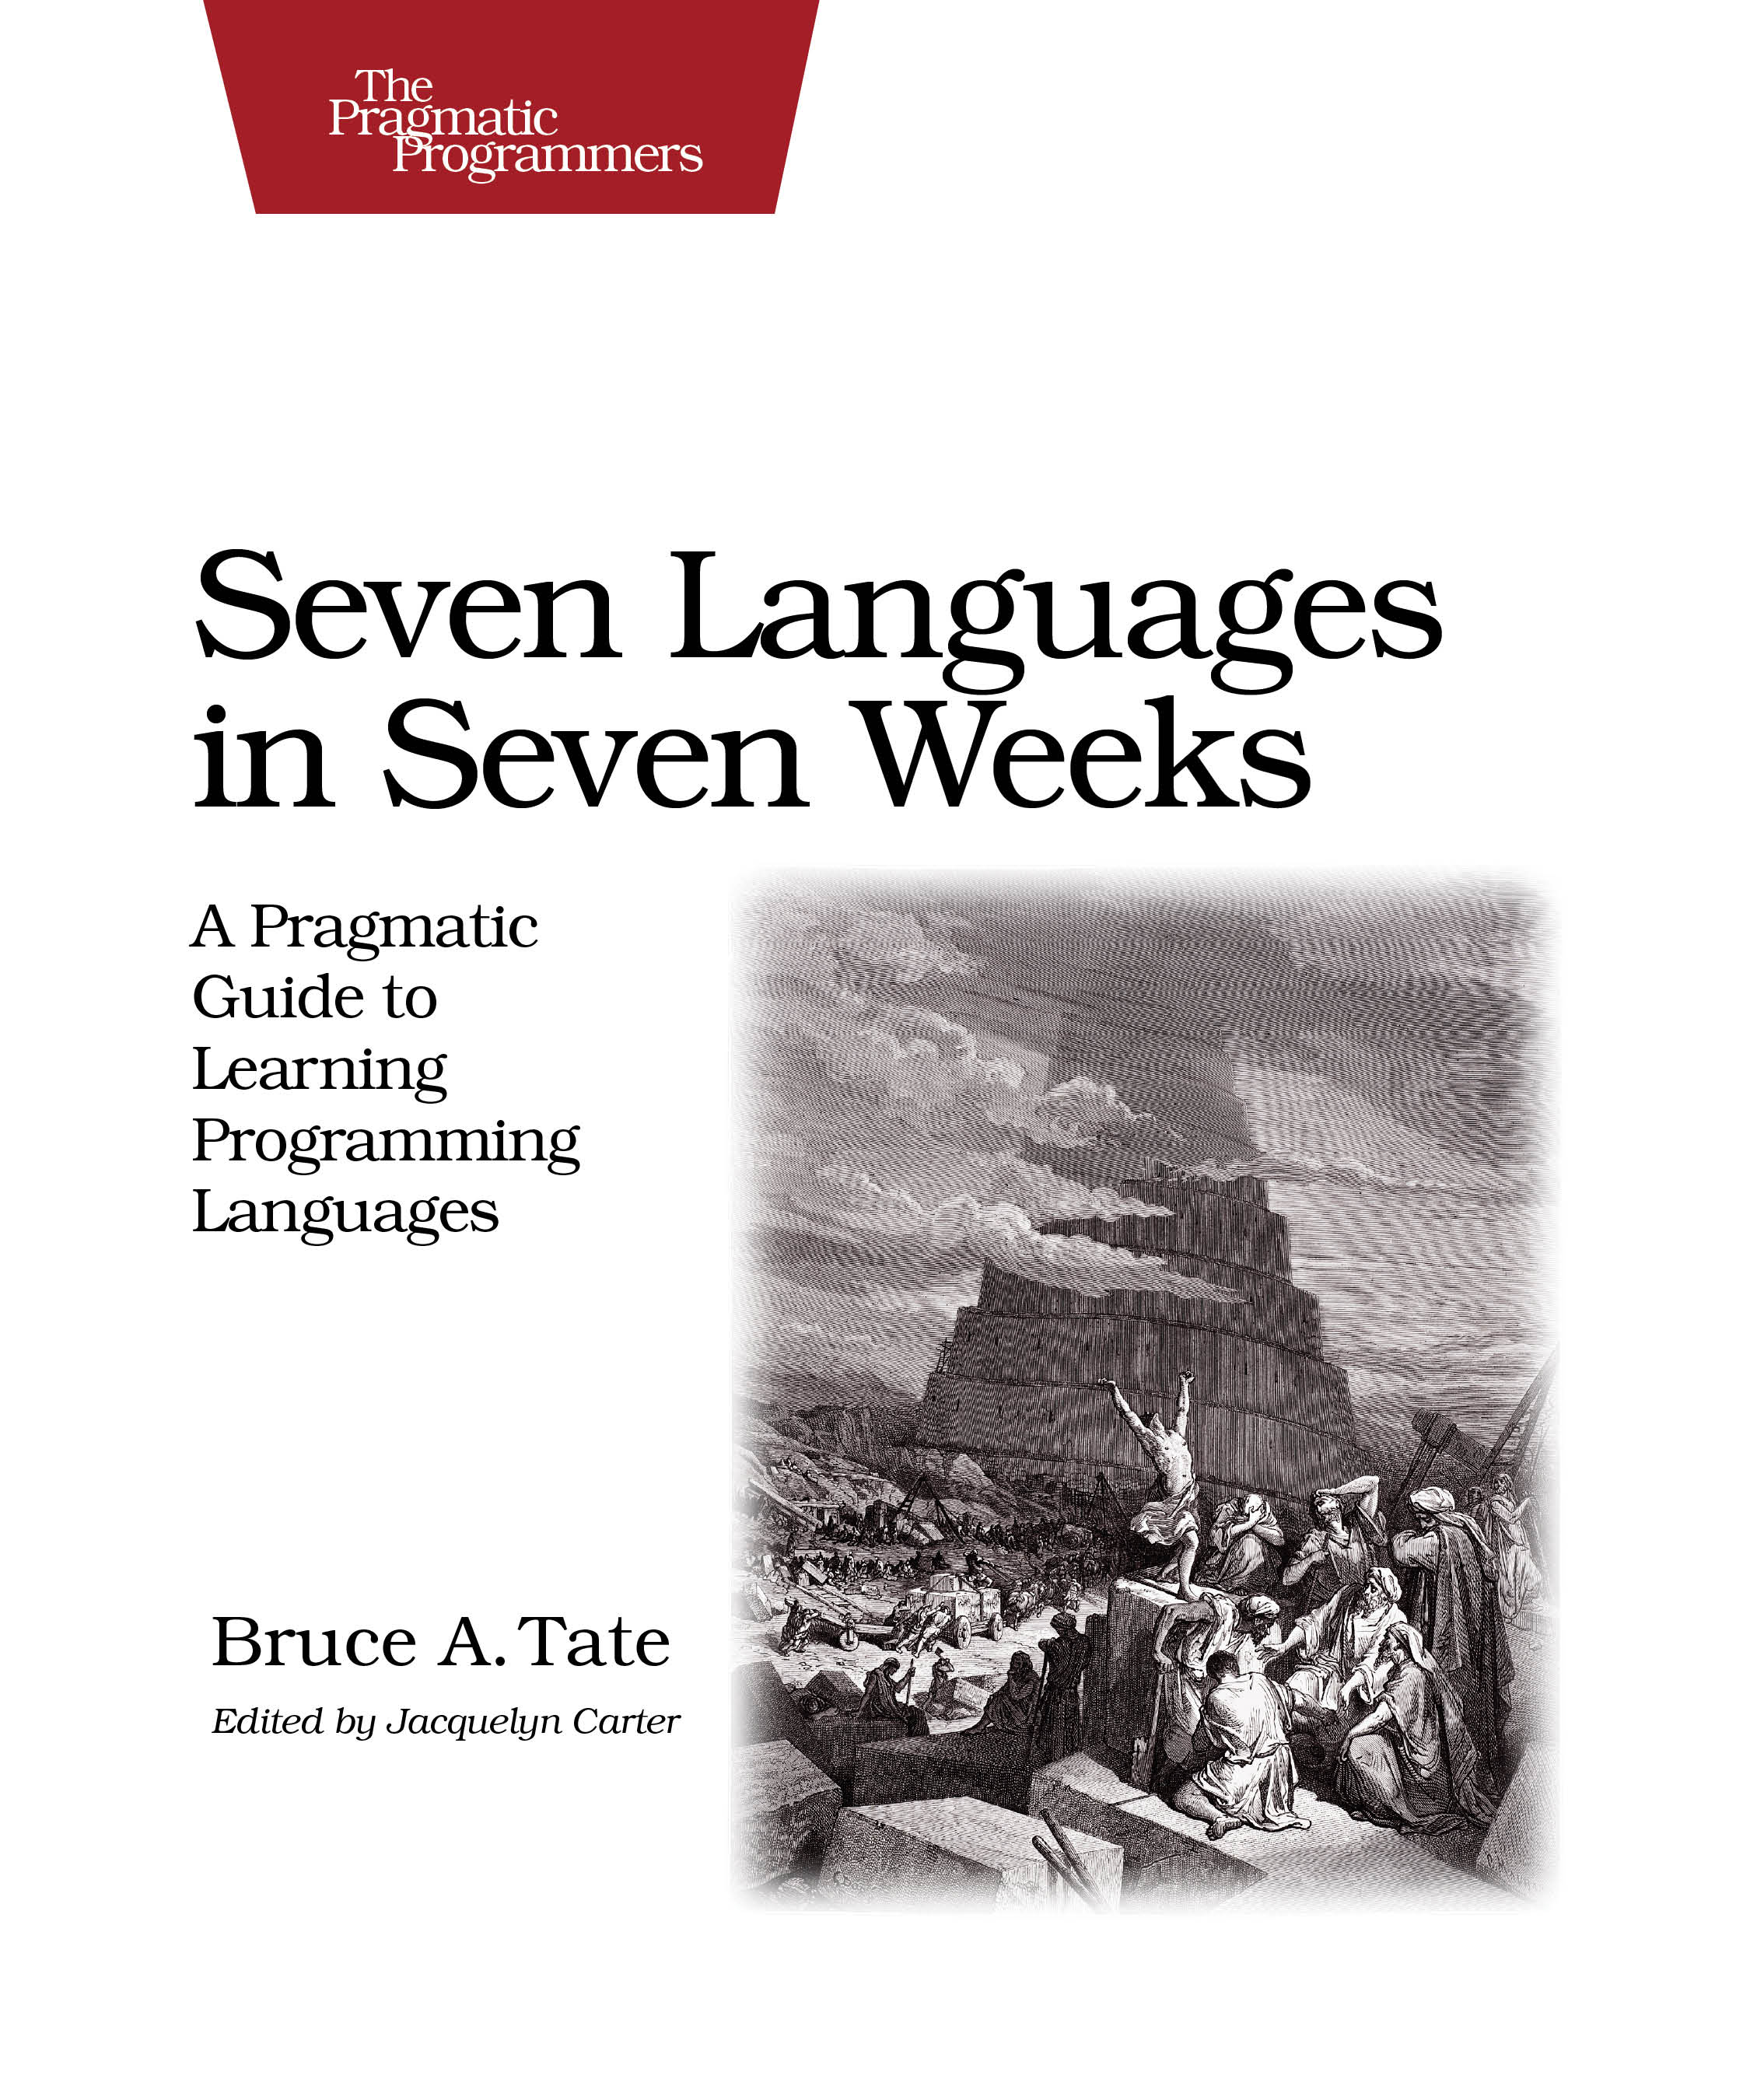
\includegraphics[height=\textheight]{slsw.jpg}}
\end{frame}

\begin{frame}
  \centerline{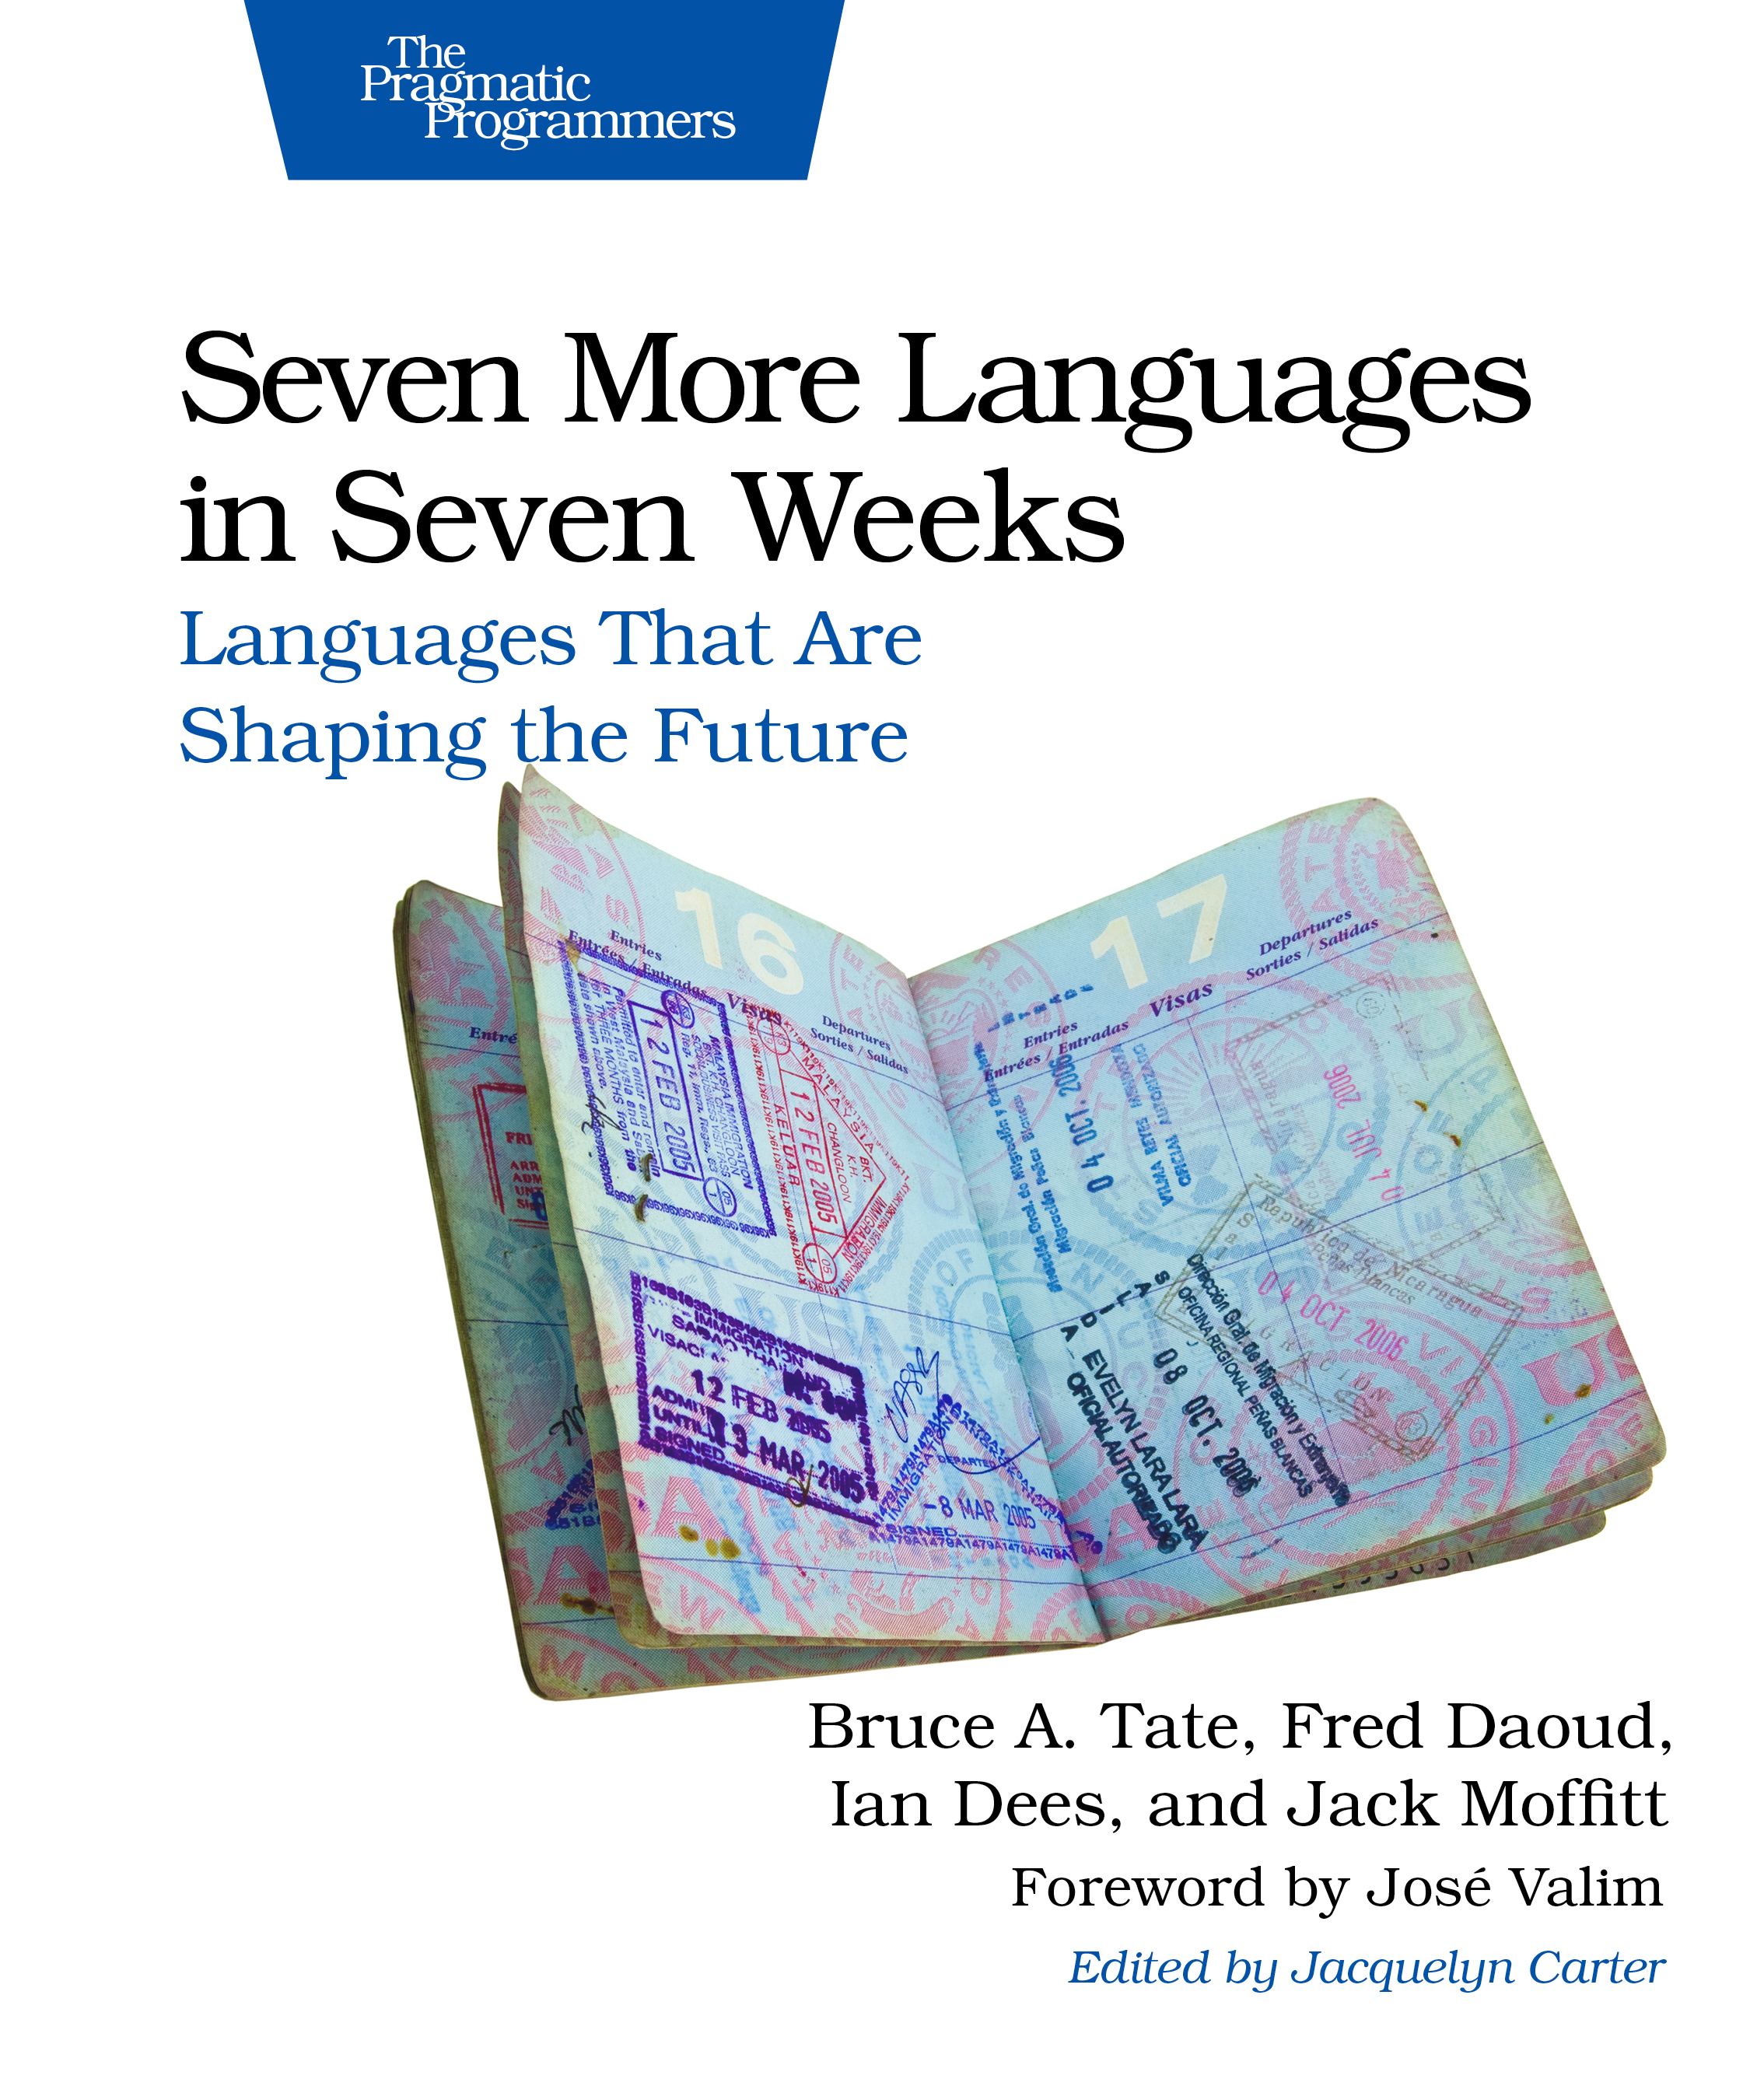
\includegraphics[height=\textheight]{smlsw.jpg}}
\end{frame}

\begin{frame}
  \centerline{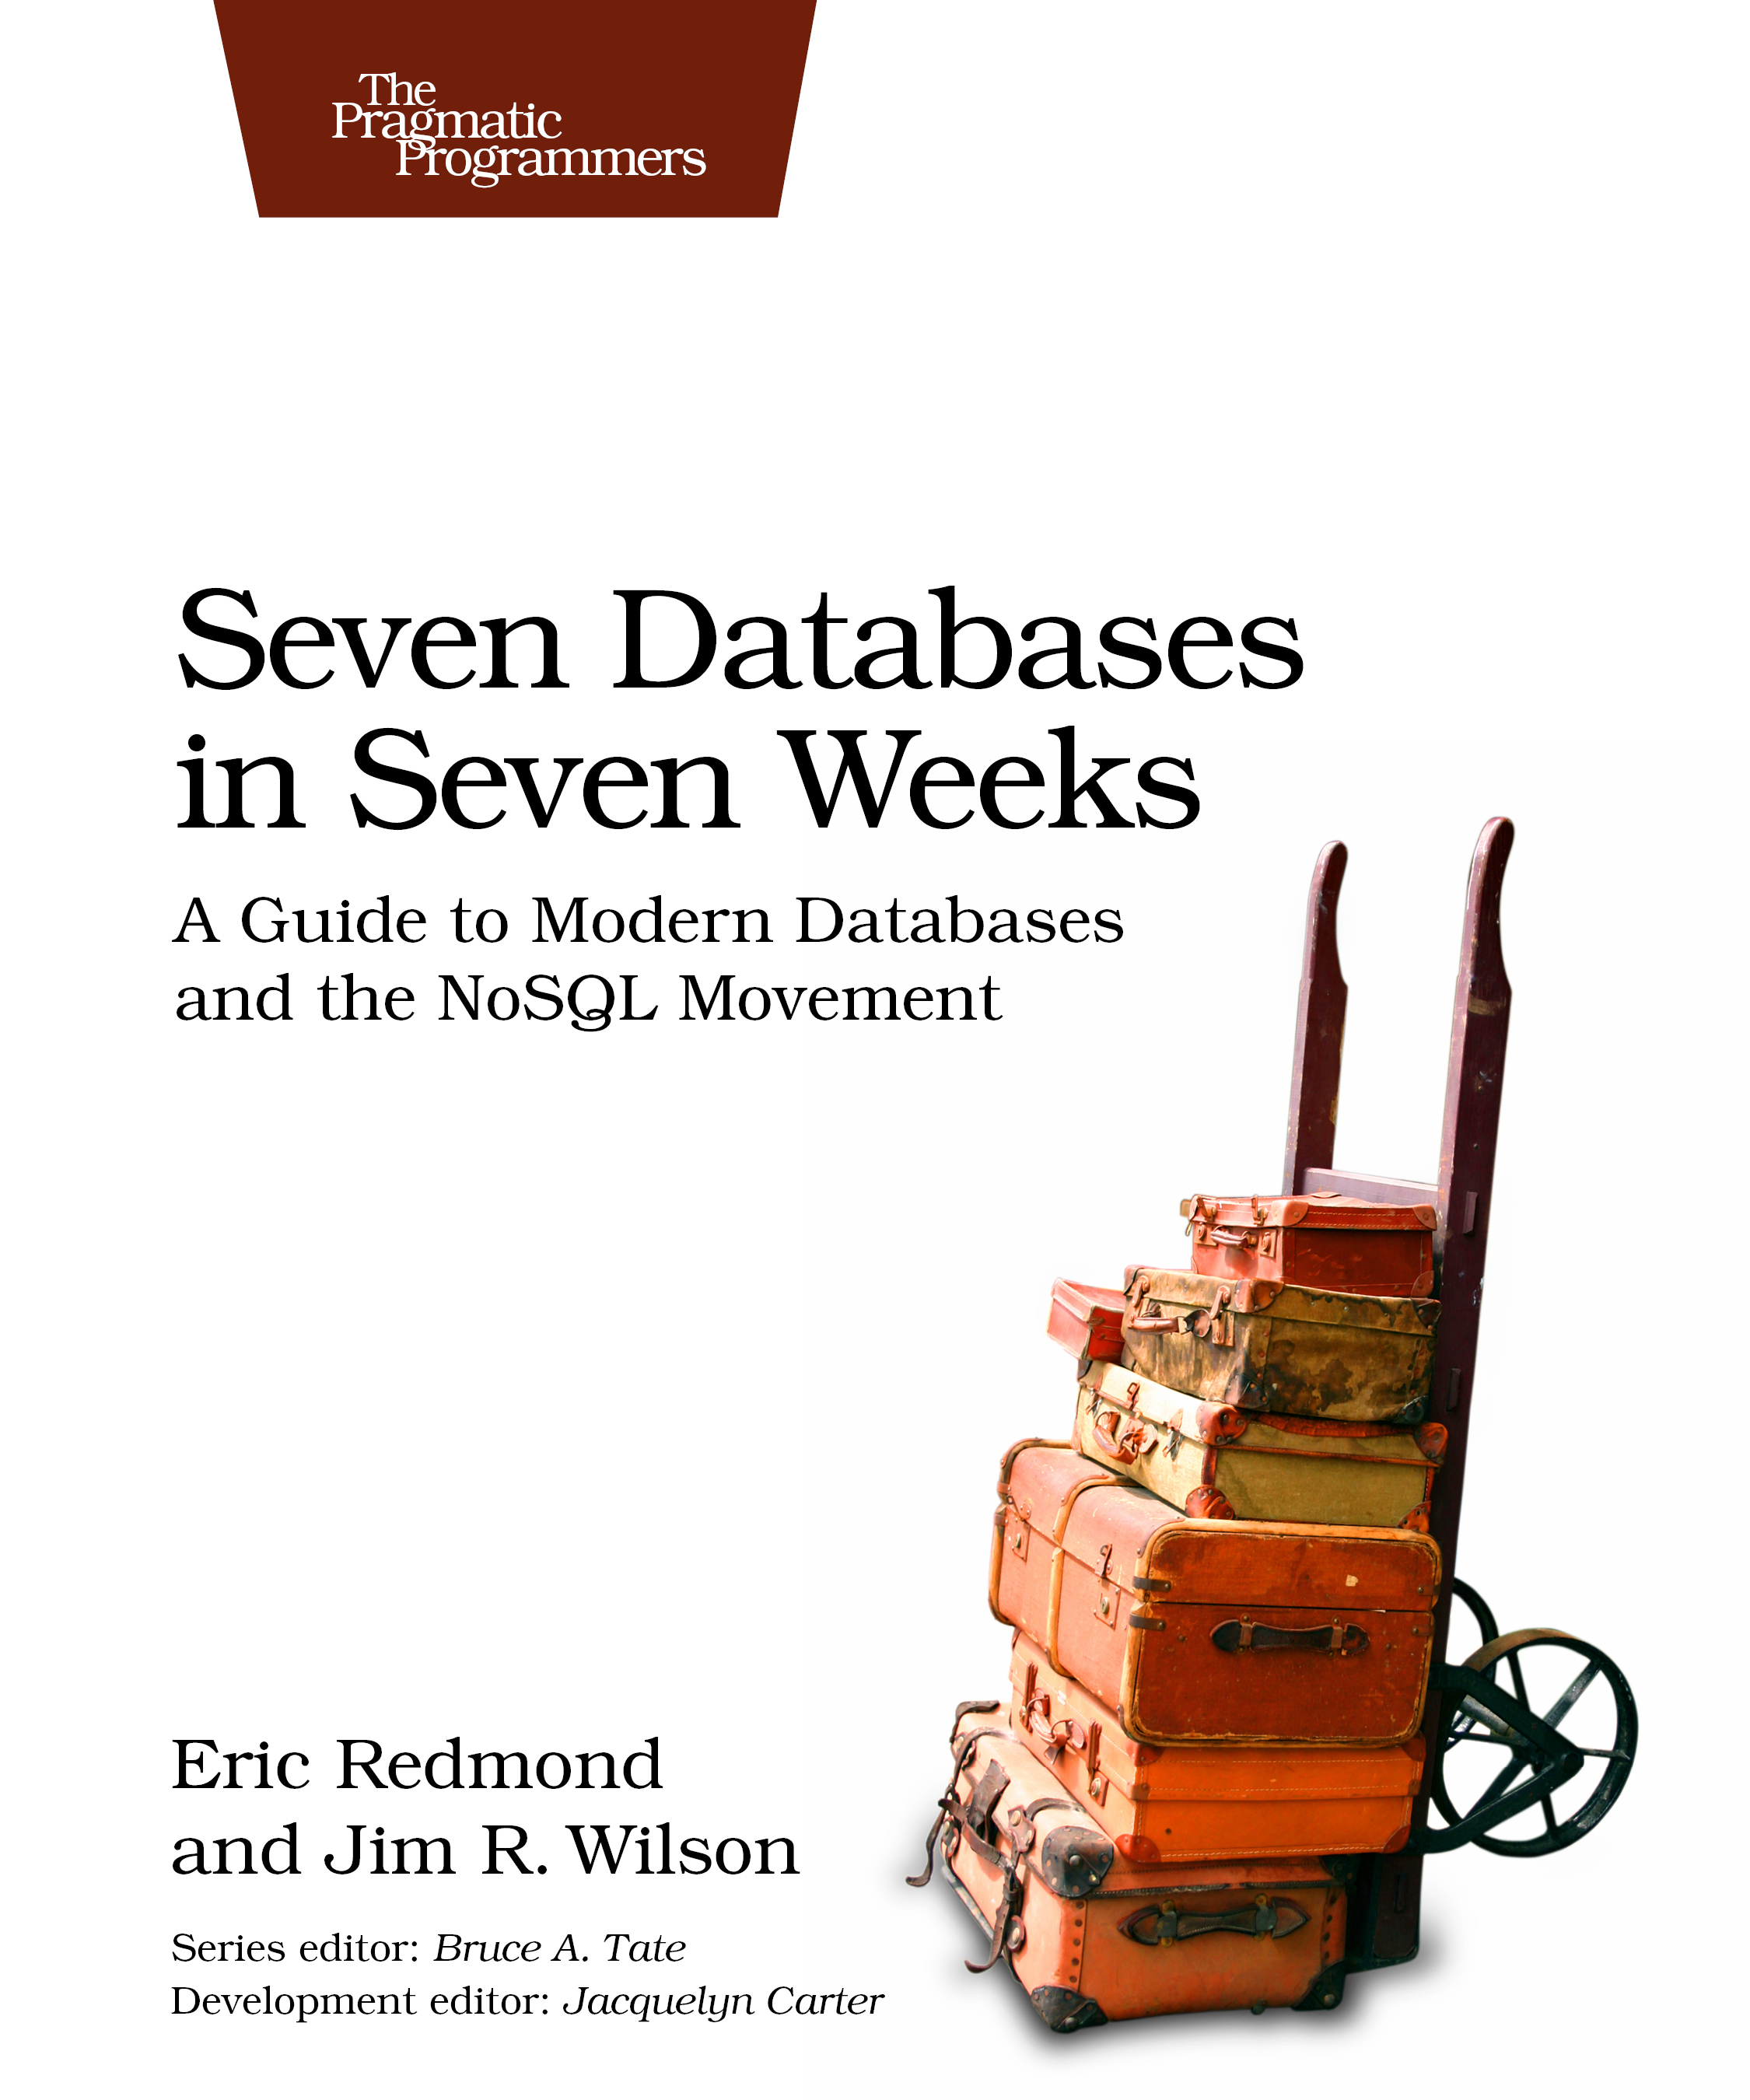
\includegraphics[width=.33\textwidth]{sdsw.jpg}
  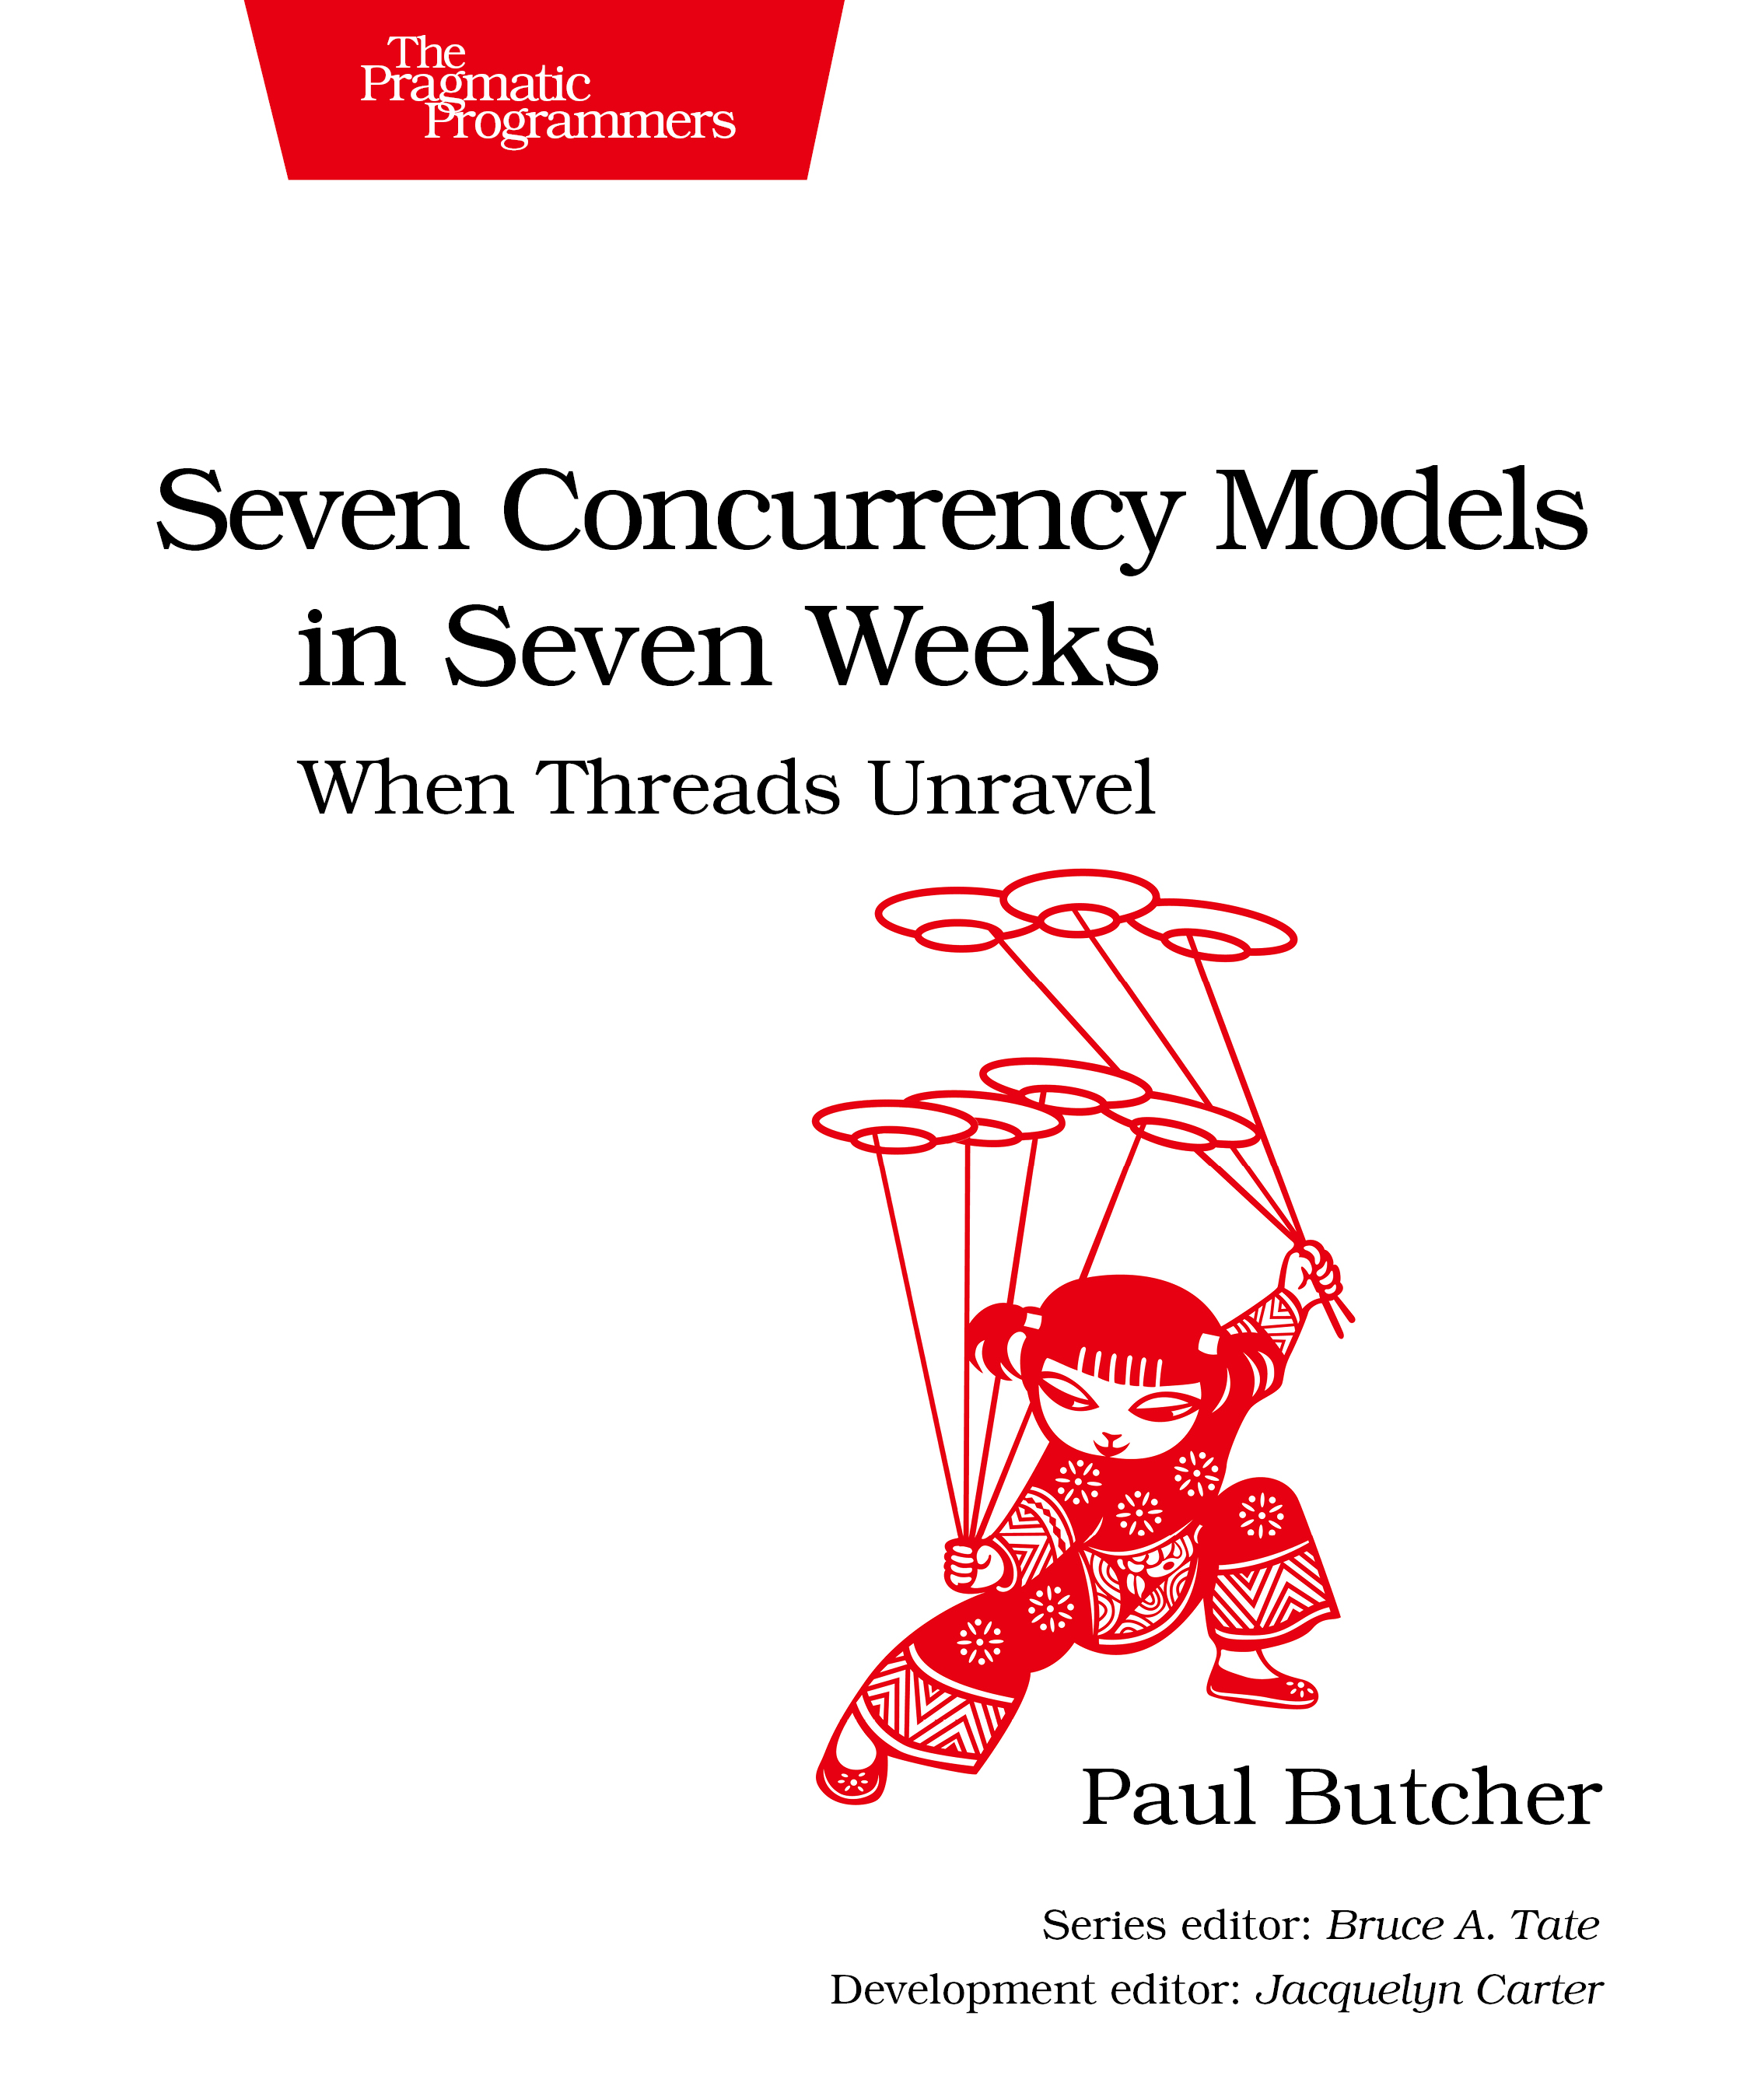
\includegraphics[width=.33\textwidth]{scmsw.jpg}
  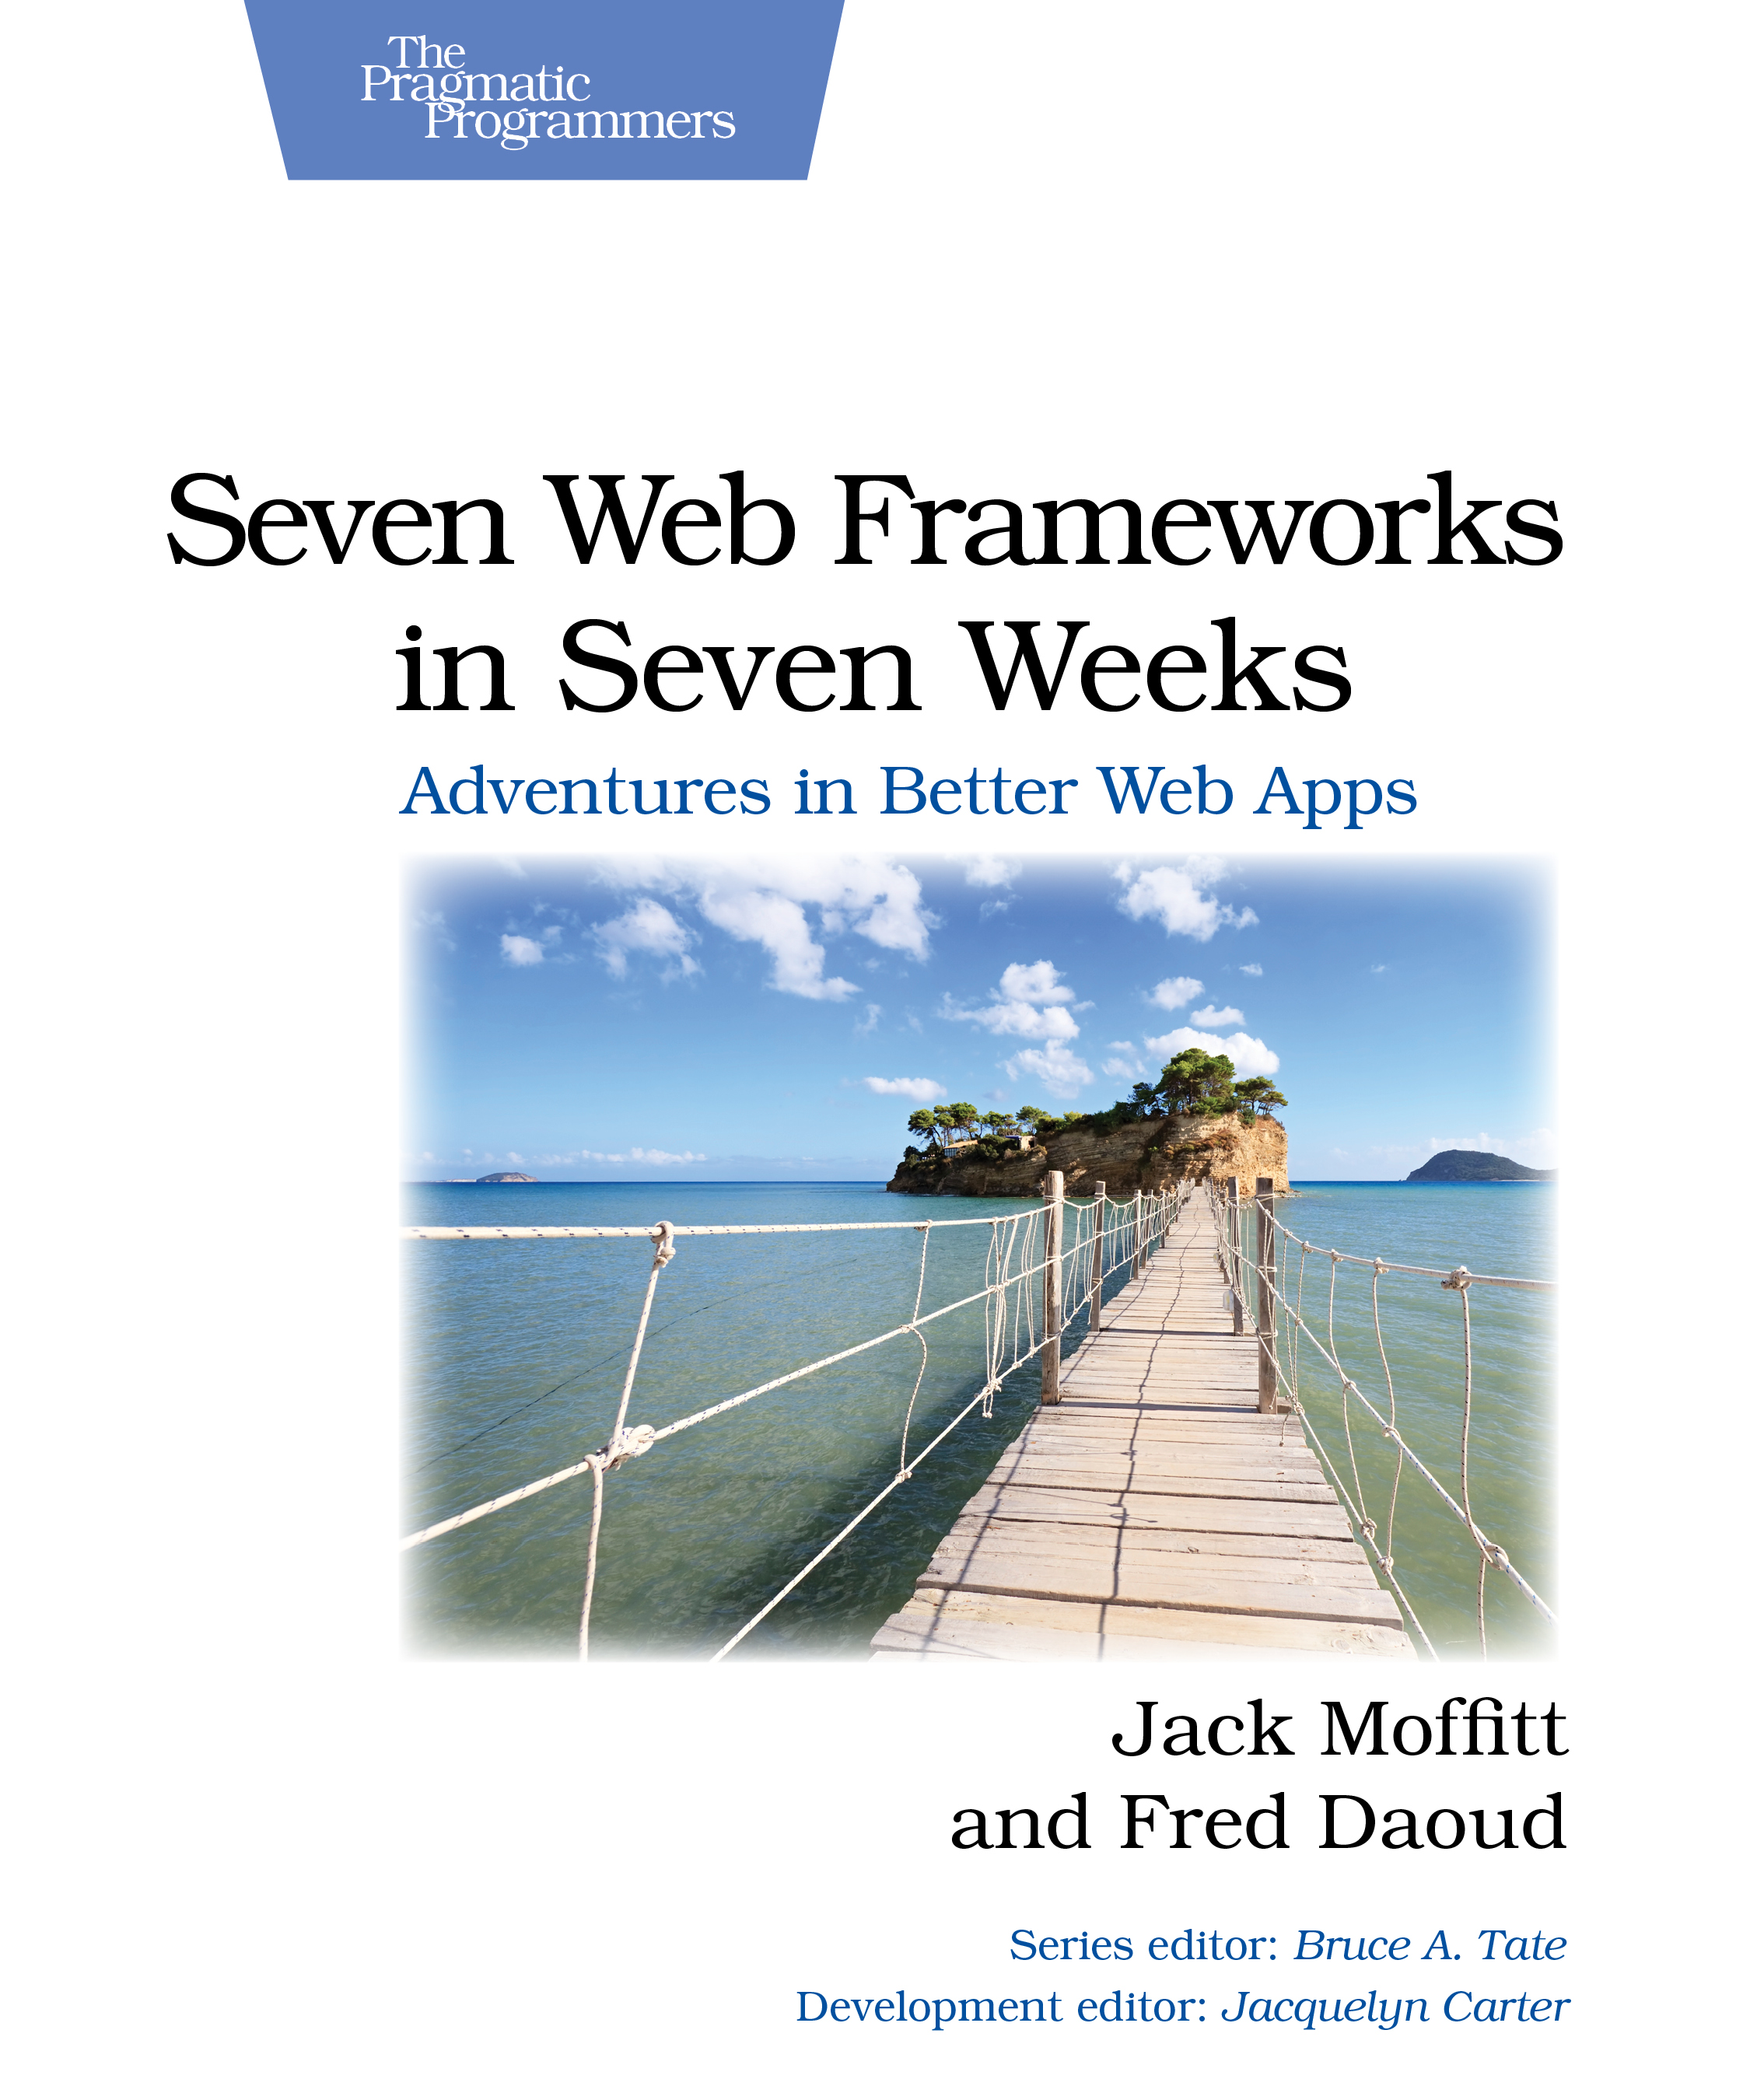
\includegraphics[width=.33\textwidth]{swfsw.jpg}}
\end{frame}

\begin{frame}
  \frametitle{Interaction between Programming Languages}
  \begin{itemize}
    \item C-based: C, C++, Go, R, Perl, Python \ldots
    \item Virtual Machine based:
    \begin{itemize}
      \item JVM: Java, Scalar, JPython, Perl 6 \ldots
      \item CLI: C++/CLI, C\#, IronPython, F\#, VB.NET, PowerShell \ldots
    \end{itemize}
    \item Interface: web service, file, database, container \ldots
  \end{itemize}
\end{frame}

\begin{frame}
  \begin{itemize}
    \item Java and R: rJava
    \item Perl and R: RSPerl
    \item Python and R: rpy2
    \item C/C++ and R: Rcpp
    \item C and Perl: perl.h
    \item Java and C/C++: JNI
  \end{itemize}
\end{frame}

\begin{frame}
  Example: Integration of R and C++\\
  see rcpp directory.
\end{frame}


\section{Software Development Process}

\subsection{Waterfall}
\begin{frame}
  \frametitle{Waterfall}
  \centerline{\includegraphics[height=.8\textheight]{waterflow.png}}
\end{frame}

\begin{frame}
  \frametitle{Case: Fibonacci Sequence Generator}
  \begin{itemize}
    \item Requirements: What is the input? Web based or Command line application?
    \item Design: technology stack, architecture, user experience \ldots
    \item Implementation: only coding? Construction
    \item Verification: testing, alpha, beta
    \item Maintenance:
  \end{itemize}
\end{frame}

\subsection{Agile Software Development}

\begin{frame}
  \frametitle{Agile Software Development}
  \begin{block}{Agile Software Development}
    Agile software development is a group of software development methods in which requirements and
    solutions evolve through collaboration between self-organizing, cross-functional teams. It
    promotes adaptive planning, evolutionary development, early delivery, continuous improvement
    and encourages rapid and flexible response to change.
  \end{block}
\end{frame}

\begin{frame}
  \frametitle{12 principles of agile software development}
  \tiny
  \begin{itemize}
    \item Customer satisfaction by rapid delivery of useful software
    \item Welcome changing requirements, even late in development
    \item Working software is delivered frequently (weeks rather than months)
    \item Close, daily cooperation between business people and developers
    \item Projects are built around motivated individuals, who should be trusted
    \item Face-to-face conversation is the best form of communication (co-location)
    \item Working software is the principal measure of progress
    \item Sustainable development, able to maintain a constant pace
    \item Continuous attention to technical excellence and good design
    \item Simplicity—the art of maximizing the amount of work not done—is essential
    \item Self-organizing teams
    \item Regular adaptation to changing circumstances
  \end{itemize}
\end{frame}

\begin{frame}
  \frametitle{Why do we need agile software development?}
  \begin{itemize}
    \item Stock trading system, military, bank \ldots
    \item Desktop softwares ship as floppy disk, CD or DVD \ldots
    \item Internet helps us update our software every minutes \ldots
  \end{itemize}
\end{frame}

\begin{frame}
  \begin{block}{Agile Methods}
    \begin{itemize}
      \item Extreme Programming
      \item Test Driven Programming
      \item Scrum
      \item \ldots
    \end{itemize}
  \end{block}
\end{frame}

\begin{frame}
  \begin{block}{Agile Practices}
    \begin{itemize}
      \item Pari programming
      \item test-driven
      \item story-driven modeling
      \item Iterative and incremental development
      \item Cross-functional team
      \item Refactoring
      \item \ldots
    \end{itemize}
  \end{block}
\end{frame}

\begin{frame}
  \frametitle{Practice: Pair Programming}
  \begin{block}{Pair Programming}
    An agile software development technique in which two programmers work together
    at one workstation
    \begin{itemize}
      \item Driver: writes codes
      \item Observer: reviews each line of code as it is typed in.
    \end{itemize}
  \end{block}
\end{frame}


\begin{frame}
  \frametitle{Practice: Pair Programming}
  \begin{block}{Fibonacci Sequence Generator}
    \begin{itemize}
      \item Input from command line argument
      \item Output to screen
      \item What will happen if the input is less than 1?
      \item What will happend if the input is more than 2000?
      \item Who is driver? Who is observer?
    \end{itemize}
  \end{block}
\end{frame}

\subsection{Refernce}
\begin{frame}
  \frametitle{Reference}
  \begin{columns}
    \begin{column}{.6\textwidth}
      \begin{itemize}
        \item Code Complete, Second Edition
        \item http://www.cc2e.com/
      \end{itemize}
    \end{column}
    \begin{column}{.4\textwidth}
      \includegraphics[width=.9\textwidth]{cc2e.jpg}
    \end{column}
  \end{columns}
\end{frame}

\section{Final Examination}
\begin{frame}
  \frametitle{Scope}
  \begin{itemize}
    \item Basic knowledge of the five programming language
    \item How to choose a programming language for your work
    \item Basic knowledge of software engineering
  \end{itemize}
\end{frame}

\begin{frame}
  \frametitle{Question Sample}
  Is it possible to implement object-oriented programming using Perl?
  \begin{itemize}
    \item Yes
    \item No
  \end{itemize}
\end{frame}

\begin{frame}
  \frametitle{Question Sample}
  Which one is not a OOP system in R?
  \begin{itemize}
    \item S3
    \item S4
    \item ROOP
    \item RC
  \end{itemize}
\end{frame}

\begin{frame}
  \frametitle{Question Sample}
  Assueme that you customer needs a website to provide genome annotation service. Choose a
  programming language for this work and explain the reason.
\end{frame}

\begin{frame}
  \frametitle{Tips}
  \begin{itemize}
    \item Don't leave blank on your answer sheet.
    \item Review the slides of this course before exam.
    \item Finish all assignments as required.
  \end{itemize}
\end{frame}

\begin{frame}
  \centerline{\Huge{Thanks!}}
\end{frame}

\end{document}
